\chapter{TINJAUAN PUSTAKA}
\vspace{4ex}

\hspace{\parindent} Demi mendukung penelitian ini, dibutuhkan beberapa teori penunjang sebagai bahan acuan dan referensi. Pada bagian ini, teori penunjang tersebut dijabarkan secara ringkas untuk menjadi dasar dalam menyelesaikan penelitian yang lebih terarah.
\vspace{2ex}

\section{\textit{Related Researches}}
\vspace{1ex}
	Pada sub bab ini dijelaskan mengenai beberapa penelitian sebelumnya yang berelasi dengan tugas akhir ini.
\vspace{1.5ex}
	
	\subsection{Proyeksi Interaktif Objek Hologram 3D menggunakan \textit{Aerial Projection}}
	\vspace{1ex}
		Penelitian ini mencoba konsep dan desain dari sistem \textit{interactive aerial projection} yang dilakukan dengan \textit{prototype demonstration}. Penelitian ini berfokus untuk menampilkan objek 3D di udara dan manipulasi objek 3D dari \textit{finger movement}. Sistem yang berhasil dibuat pada penelitian ini terdiri dari \textit{Reconstruction of 3D Object} dengan menggunakan \textit{pyramid hologram device}, \textit{Projection of 3D Hologram Object in the Mid-Air} dengan \textit{concave mirror} berbentuk parabola, dan \textit{Interactive Manipulation of 3D Hologram Object} dengan \textit{leap motion}. Sistem ini berhasil dibangun meskipun dengan \textit{workspace} dan interaksi yang terbatas.\cite{mahfud2016interactive}
	\vspace{1.5ex}

	\subsection{Pembuatan Dataset \textit{Hand Gesture} menggunakan \textit{Leap Motion}}
	\vspace{1ex}
		Penelitian ini berkaitan dengan \textit{3D dynamic gesture recognition} berdasarkan posisi ujung jari dan telapak 	tangan. Penelitian ini berfokus pada proses pembuatan dataset baru yang digunakan dalam penyusunan sebuah sistem kontrol. Dataset yang dibuat berpedoman dari \textit{general commands} (yang umum diterapkan pada \textit{leap motion}) sebagai parameter \textit{training}. Metode ini berhasil diterapkan dengan nilai akurasi yang cukup tinggi, sehingga dapat diterapkan untuk mengembangkan \textit{feature} baru.\cite{ameur2016comprehensive}
	\vspace{1.5ex}
	
	\subsection{Faktor-faktor yang Mempengaruhi \textit{Interactive 3D Holographic Projection System} untuk \textit{Experiential Learning}}
	\vspace{1ex}
		Penelitian ini berkaitan dengan informasi yang dapat disajikan dalam mendukung \textit{interactive ecperiental learning} yang menghasilkan pedoman untuk \textit{3D display and control of interactive experience}. Faktor-faktor tersebut dinyatakan dalam tabel \ref{tab:faktor-nilaiguna-3d}.
		\vspace{-2ex}
		\begin{table}[!htb]
			\caption{Faktor-faktor yang Memengaruhi Nilai Guna \textit{3D Holographic Projection System}}
			\label{tab:faktor-nilaiguna-3d}
			\vspace{-2ex}
			\begin{center}
			\begin{tabular}{|C{0.4cm}|L{2.2cm}|L{6.3cm}|}
				\hline
				\textbf{No} & \multicolumn{1}{c|}{\textbf{Item}} & \multicolumn{1}{c|}{\textbf{Deskripsi}}\\ \hline
				1.& \textit{Image Space}               & Ukuran dari  objek pada \textit{holographic projection}                             \\ \hline
				2.& \textit{Icon Shape}                & Bentuk dan ukuran simbol penyusun \textit{interface}                                 \\ \hline
				3.& \textit{Cursor Reminder}           & Efek pergerakan kursor pada \textit{interface}                                       \\ \hline
				4.& \textit{Rich Contents}             & Kompleksitas informasi dari \textit{learning objective} yang ingin disampaikan \\ \hline
				5.& \textit{Level Guider}              & Kesesuaian \textit{interface}  dengan scene yang sedang berjalan                          \\ \hline
				6.& \textit{Compatible Gestures}       & Sensitivitas dan kesesuaian respons terhadap \textit{gesture} yang diberikan               \\ \hline
				7.& \textit{Sensitive Cursors}         & Sensitivitas dari pergerakan kursor terhadap \textit{interface}                           \\ \hline
				8.& \textit{Adjustable Function}       & Kemampuan \textit{user} dalam mengatur \textit{control function}                          \\ \hline
				9.& \textit{Sound Feedback}            & \textit{Feedback} dari \textit{interface} saat ada instruksi maupun \textit{click sound}  \\ \hline
				10.& \textit{Background Music (BGM)}    & Musik atau lagu yang diputar saat suatu \textit{scene} sedang berlangsung                 \\ \hline
				11.& \textit{Switching Effect}          & Efek \textit{visual animation} saat perpindahan \textit{scene}                            \\ \hline
				12.& \textit{Ambient Brightness}        & Tingkat kecerahan \textit{environment} sekitar saat \textit{holographic projection }      \\ \hline
			\end{tabular}
			\end{center}
		\end{table}
	\vspace{2ex}
	
	Penelitian ini menghasilkan kesimpulan bahwa faktor-faktor ini dapat membantu penyampaian informasi lebih efektif dan efisien. Sistem \textit{3D holographic projection interactive} ini dapat memberikan output yang berbeda dibandingkan dengan pembelajaran konvensional dengan dengan buku. Penelitian ini pun juga mengemukakan bahwa hasil dari penelitian ini dapat diterapkan pada pembelajaran digital seperti \textit{virtual museum exhibition}.\cite{huang2018factors}
\vspace{2ex}

\section{Visualisasi Objek 3D}
\vspace{1ex}
	Visualisasi adalah suatu metode rekayasa dalam menampilkan sebuah informasi, baik gambar, diagram, ataupun animasi. Dalam memvisualisasikan objek 3D (selanjutnya disebut model 3D), yang perlu diperhatikan adalah bagaimana objek tersebut berhasil merepresentasikan objek di dunia nyata. Suatu model 3D tidak menjamin dapat memberikan ilusi mirip dengan objek aslinya yang dilihat dengan penginderaan manusia (\textit{real world}). Pada dasarnya, model 3D merupakan hasil pemrosesan dan pemberian efek cahaya terhadap bentuk 2D sehingga objek tersebut seolah-olah memiliki kedalaman (sumbu x, y, dan z). Pencahayaan ini mempengaruhi realsitas suatu model 3D. Tanpa adanya pencahayaan, model 3D tidak memiliki bayangan dan terlihat tidak memiliki kedalaman. 
	\begin{comment}
		Perbandingan model 3D yang diberikan pencahayaan maupun tidak ditunjukkan pada gambar \ref{fig:model3d_cahaya}.
	\begin{figure} [H]
	\includegraphics[scale=0.4]{img/bab2/model3d_cahaya.png}
	\caption{Perbandingan efek pencahayaan pada model 3D. \colorbox{yellow}{model awal > model dgn pencahayaan diubah2 posisinya}}
	\label{fig:model3d_cahaya}
	\end{figure}
	\end{comment}
			
	Selain pencahayaan, efek dan detail yang diberikan pada permukaan objek juga membedakan realistas antar model 3D. \textit{Texturing} berfungsi membuat sebuah objek menjadi lebih nyata seperti aslinya dengan memberikan karakteristik terhadap permukaan objek. Objek nyata tidak selalu memiliki permukaan yang halus atau rata, maka untuk menampilkan detail permukaan pada model 3D dibutuhkan \textit{UV map}. \textit{UV map} digunakan untuk menekankan bentuk detail objek dimana mencakup pengaturan bayangan, pewarnaan, dan bentuk teksturnya sehingga dapat memberikan efek realistis pada model 3D tanpa harus dimodelkan bentuknya karena \textit{uv mapping} adalah proses 'penempelan' 2D image terhadap permukaan model 3D. Tingkat detail model 3D disesuaikan dengan peruntukannya karena semakin detail modelnya, maka dibutuhkan \textit{hardware} dengan spesifikasi yang lebih canggih agar program tersebut dapat berjalan dengan baik. Contoh dari objek sebelum dan setelah \textit{uv mapping} ditunjukkan pada gambar \ref{fig:model3d_tekstur}.
	\begin{figure} [H]
		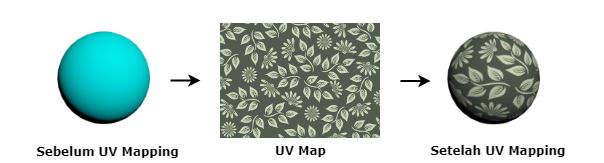
\includegraphics[scale=0.5]{img/bab2/model3d_tekstur.png}
		\caption{Objek sebelum dan setelah\textit{uv mapping}\cite{uvmap}.}
		\label{fig:model3d_tekstur}
	\end{figure}
\vspace{2ex}
	
\section{Proyeksi Hologram}
\vspace{1ex}
	Holografi (\textit{holography}), berasal dari bahasa Yunani "\textit{Holos}" berarti seluruh dan "\textit{Graphe} berarti tulisan, adalah sebuah metode yang merekam cahaya yang tersebar dan merekonstruksi pola cahaya tersebut seolah-olah membentuk suatu objek \cite{akshay_2015}. Objek yang memiliki lebar (\textit{width}), ketinggian (\textit{height}) dan kedalaman (\textit{depth}) ini dikenal sebagai objek tiga dimensi. Objek yang dihasilkan holografi dikenal sebagai hologram, yaitu objek atau \textit{image} yang dibentuk berdasarkan penyebaran/pembelokan (difraksi) pancaran cahaya. Cahaya yang dikeluarkan oleh proyektor atau alat pemancar lain akan dibelokkan dan berinterferensi dengan cahaya lain yang saling menguatkan dan membentuk pola yang dapat dilihat. Teknologi hologram yang sederhana mengadopsi teknik \textit{Pepper’s Ghost Illusion} oleh John Henry Pepper (1821-1900). \textit{Pepper’s Ghost Illusion} adalah teknik yang diterapkan pada teater untuk memberikan efek objek yang tidak nyata seperti transparan layaknya hantu. Objek transparan ini dihasilkan dari objek atau aktor yang terletak di \textit{blind spot} penonton, dimana akan dipancarkan cahaya dan dipantulkan melalui sebuah kaca yang dipasang 45° di depan penonton. Sehingga hasil pemantulannya dimanfaatkan sebagai ‘aktor’ hantu yang dilihat oleh penonton dan memainkan peran sesuai cerita\cite{vishnu2017hologram}.
	
	Hologram terbentuk karena adanya interferensi (interaksi tumpang tindih pada suatu titik tertentu) atau penggabungan cahaya antara \textit{reference beam} dan \textit{object beam}. Sinar laser mengarah ke \textit{beam splitter} terbagi menjadi dua \textit{reference beam} \cite{akshay_2015}. Salah satunya diteruskan ke objek terkait menjadi \textit{object beam}. Keduanya (\textit{reference beam} dan \textit{object beam}) jatuh pada di sebuah medium dan memunculkan bentuk hologram dari objek tersebut. Jika ada cahaya lain yang koheren dengan laser, maka cahaya ini dapat memengaruhi objek hologram yang dibentuk. Sehingga perlu meminimalisir adanya cahaya lain yang dapat mengganggu. Ilustrasi terbentuknya hologram ditampilkan pada gambar \ref{fig:hologram_kerja}.
	\begin{figure} [H]
		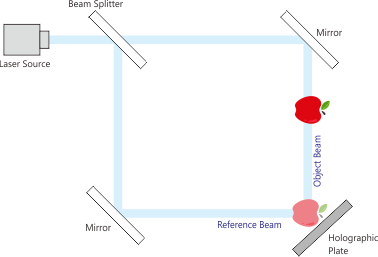
\includegraphics[scale=0.4]{img/bab2/hologram_kerja.png}
		\caption{Cara kerja hologram.}
		\label{fig:hologram_kerja}
	\end{figure}
	
	Hal yang dibutuhkan untuk menciptakan bentuk hologram adalah metode bagaimana objek asli tersebut dapat direkonstruksi dalam bentuk hologram, salah satu media yang banyak digunakan adalah \textit{pyramid hologram}. \textit{Pyramid hologram} adalah potongan media tembus pandang yang disusun dalam bentuk piramida dimana dapat memantulkan objek asli pada sebuah titik. Setiap sisi piramida memantulkan (refleksi) objek yang ditampilkan pada  monitor yang terletak di bawahnya, sehingga semua hasil pemantulan menyebabkan ojek 3D dapat dilihat dari setiap sisi. Hasil yang diberikan pun  menciptakan ilusi objek 3D yang muncul di udara, tepatnya di sisi bagian dalam piramida tersebut. Faktor ini menyebabkan besarnya objek hologram yang dihasilkan tergantung dari besarnya piramida dan monitor yang digunakan. Pemilihan jenis dan ketebalan bahan piramida dapat menentukan bentuk hologram yang dibangun. Semakin tebal bahannya, maka semakin buram (blur) objek hologram yang didapat dikarenakan adanya pemantulan berulang\cite{hologrampyramid}. Beberapa \textit{pyramid hologram} yang banyak digunakan adalah piramida 1 sisi, 3 sisi, dan 4 sisi. Berbeda jenis piramid yang digunakan maka \textit{hologram video} yang diputar pun berbeda-beda, dimana objek asli harus menghadap sisi piramida\cite{mahfud2016interactive}. Ketiganya memiliki kelebihan dan kekurangannya masing-masing.
	
	\subsection{Piramida 1 Sisi}
	\vspace{1ex}
	\textit{Pyramid hologram} 1 sisi adalah yang paling sederhana. Hanya dapat memantulkan dari 1 sisi menyebabkan objek hologram yang dihasilkan memiliki ukuran yang paling besar di antar jenis-jenis yang lain. Sama seperti pada \textit{Pepper’s Ghost Illusion}, objek asli yang ditampilkan pada monitor diletakkan pada salah satu sisi piramida membentuk sudut 45° dan hasil hologramnya muncul seolah-olah berada di luar piramida. Bentuk \textit{hologram video} yang diputar pun hanya menampilkan 1 objek yang diposisikan di tengah monitor dan hasil yang diperoleh seperti gambar \ref{fig:piramid1}.
	\begin{figure} [H]
		\subfloat[Bentuk piramida 1 sisi\cite{fotop1}.]{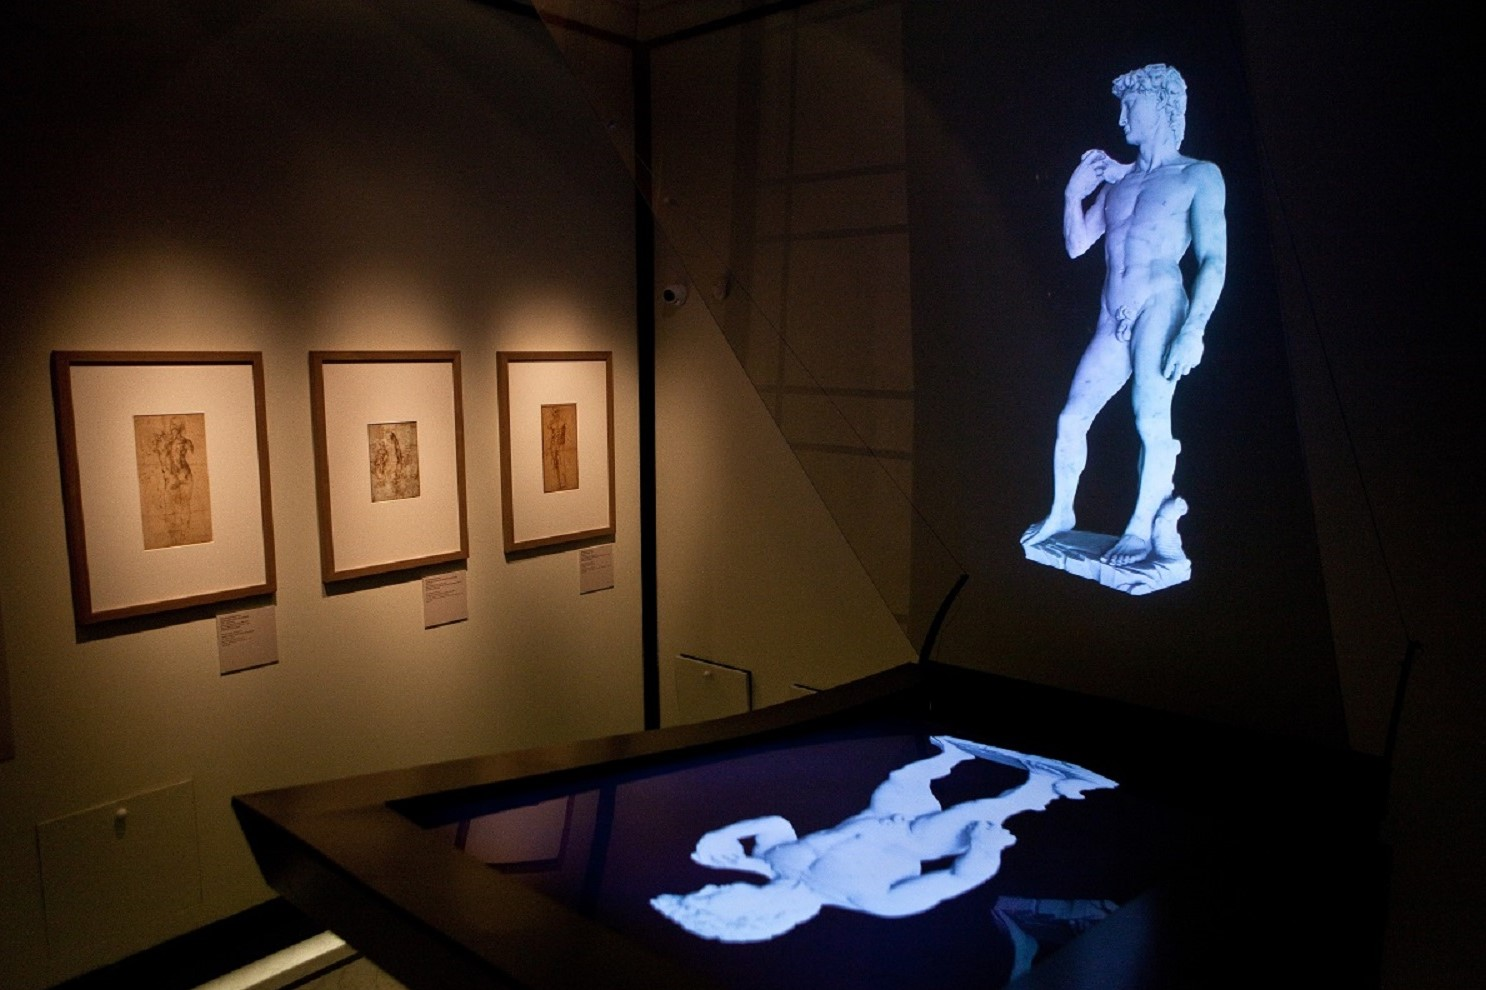
\includegraphics[width=0.47\textwidth]{img/bab2/p1_foto.jpg}}
		\hspace{0.1em}
		\subfloat[Video untuk piramida 1 sisi\cite{videop1}.]{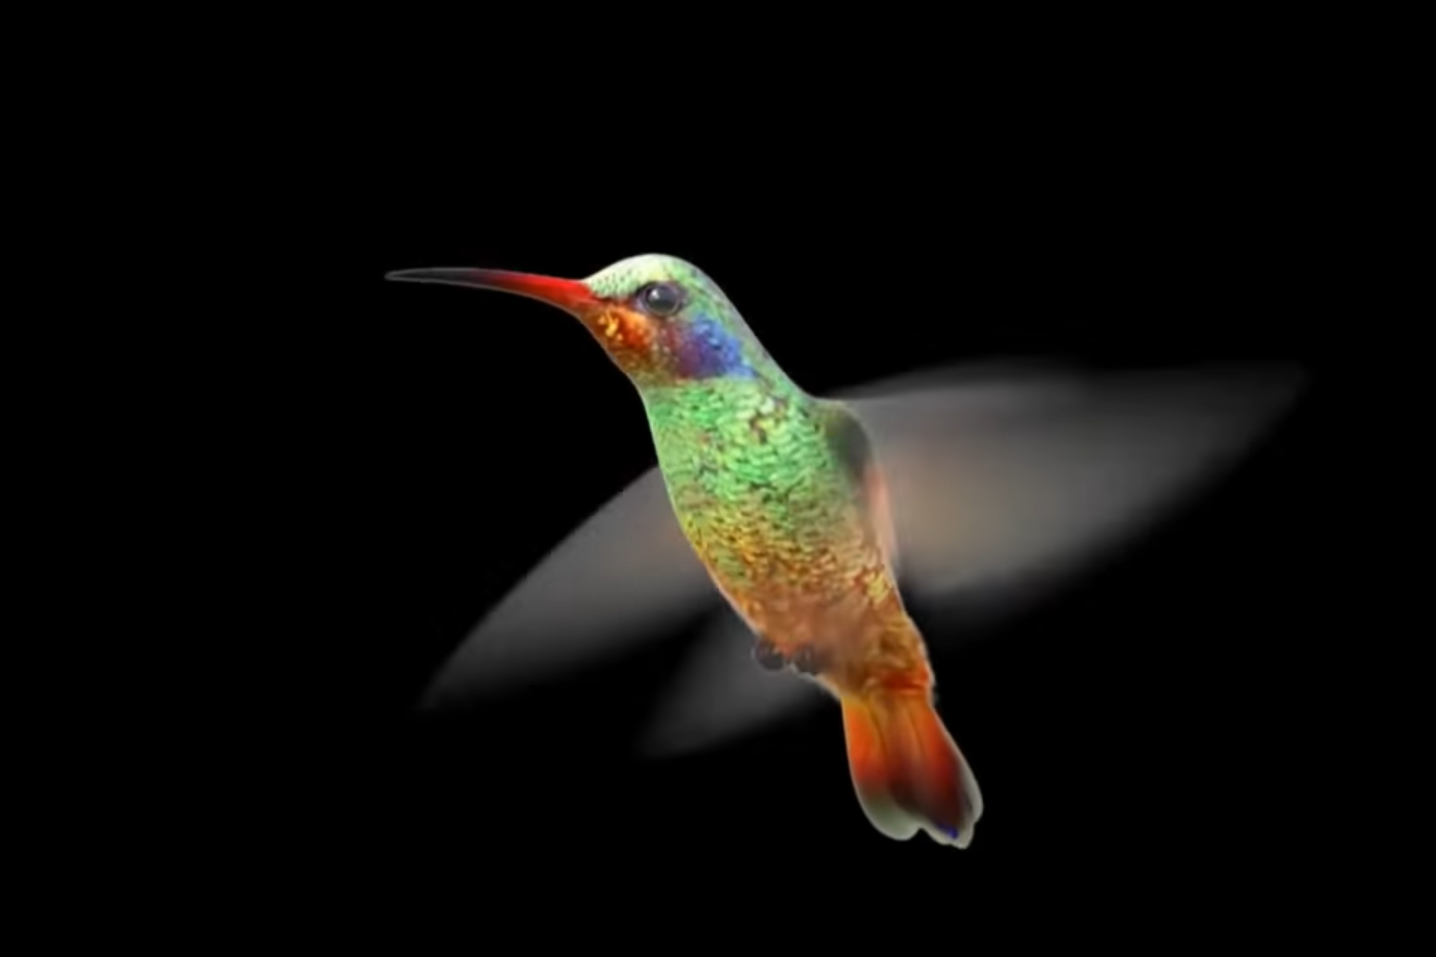
\includegraphics[width=0.47\textwidth]{img/bab2/p1_video.png}}
		\caption{Piramida 1 sisi}
		\label{fig:piramid1}
	\end{figure}
	\vspace{1.5ex}
	
	\subsection{Piramida 3 Sisi}
	\vspace{1ex}
	\textit{Pyramid hologram} 3 sisi adalah 'setengah' dari piramida 4 sisi. Piramida jenis ini memungkinkan objek hologram dapat dilihat dari 3 sisi sejauh 270° dengan salah satu sisinya tertutup, sehingga banyak diaplikasikan untuk memberikan animasi pada objek koleksi yang dipajang\cite{ironman}. Berbeda dengan kedua jenis yang lain, kebanyakan piramida jenis ini digunakan untuk memutar \textit{hologram video} dengan posisi monitor yang menghadap ke bawah. Bentuk \textit{hologram video} yang diputar memiliki 3 objek yang membentuk huruf Y (antar objek membentuk sudut sebesar 60°) dan hasil yang diperoleh seperti gambar \ref{fig:piramid3}. Menampilkan 3 objek dalam 1 monitor menyebabkan objek hologram yang ditampilkan tidak sebesar pada piramid 1 sisi.
	\begin{figure} [H]
		\subfloat[Bentuk piramida 3 sisi\cite{fotop3}.]{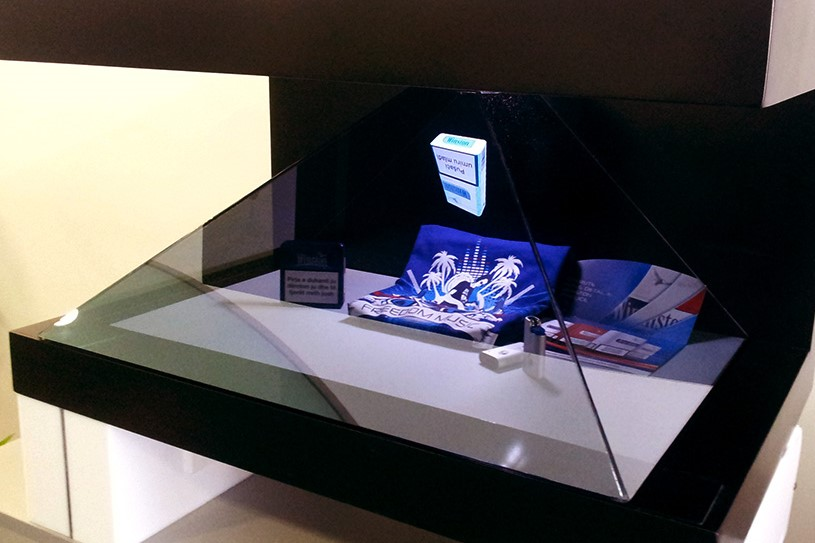
\includegraphics[width=0.47\textwidth]{img/bab2/p3_foto.jpg}}
		\hspace{0.1em}
		\subfloat[Video untuk piramida 3 sisi\cite{videop3}.]{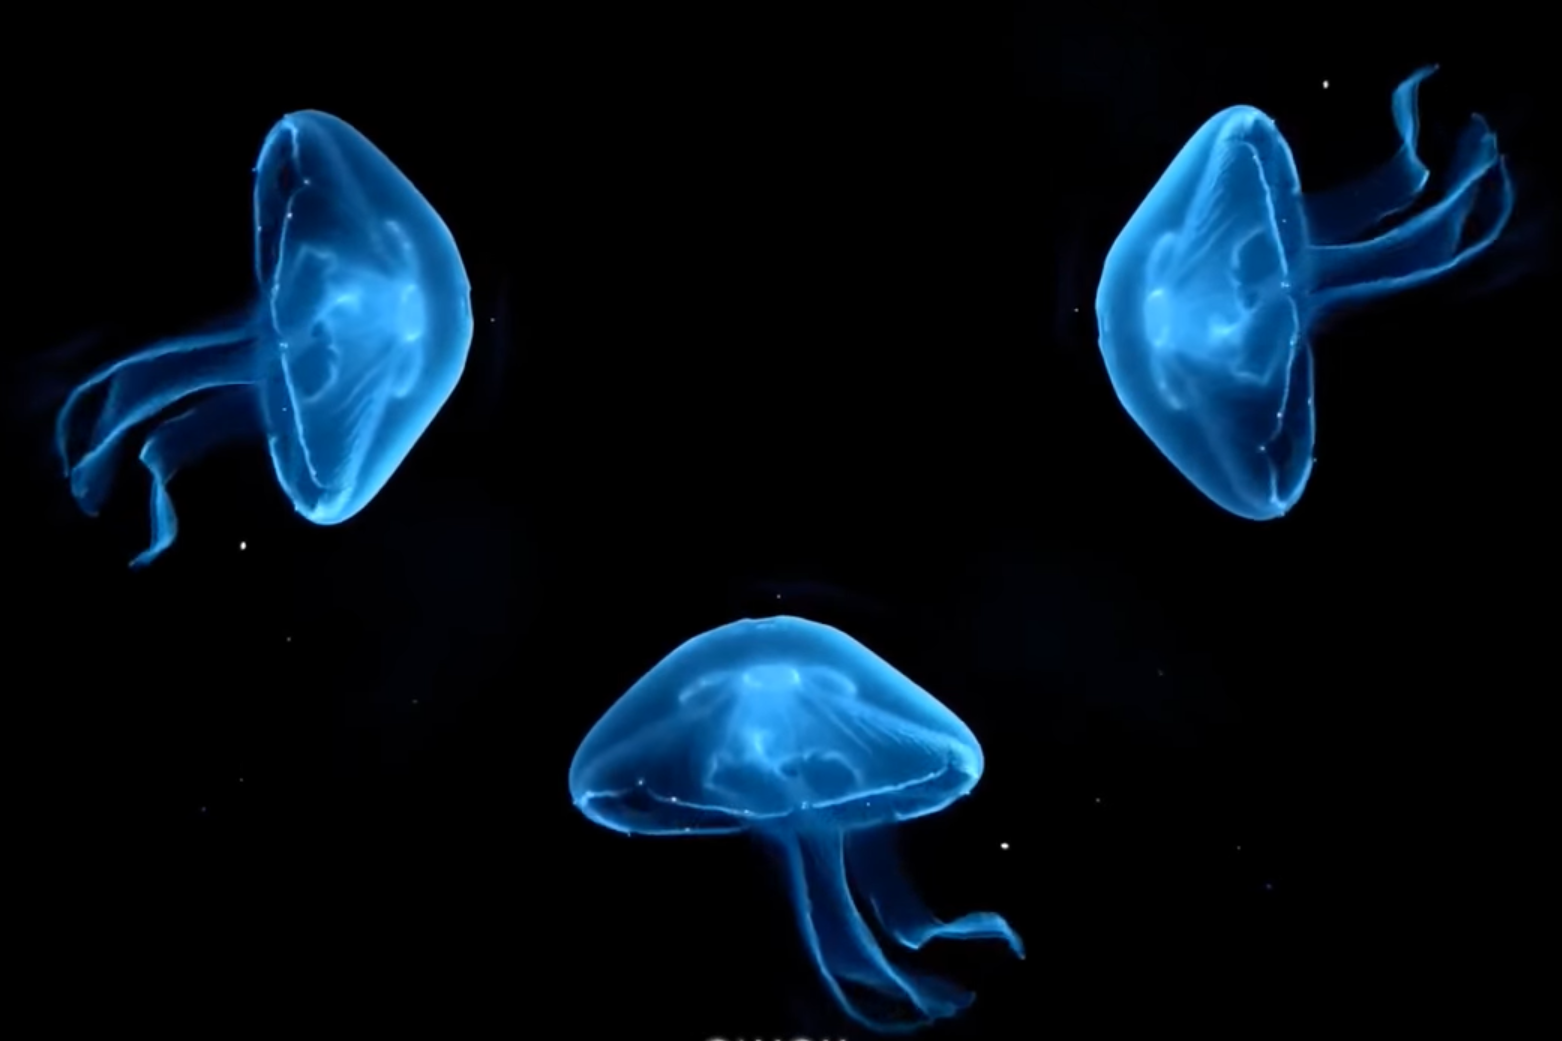
\includegraphics[width=0.47\textwidth]{img/bab2/p3_video.png}}
		\caption{Piramida 3 sisi}
		\label{fig:piramid3}
	\end{figure}
	\vspace{1.5ex}
	
	\subsection{Piramida 4 Sisi}
	\vspace{1ex}
	\textit{Pyramid hologram} 3 sisi adalah jenis piramida yang paling umum dikenal. Karena ke empat sisi yang simetris (6 : 3.5 : 1), piramida jenis ini banyak dibuat dengan bahan yang mudah dan dimanfaatkan untuk memutar \textit{hologram video} pada \textit{smartphone}\cite{tutorialpiramid}. Piramida 4 sisi ini dapat digunakan untuk memutar \textit{hologram video} dengan monitor menghadap ke atas maupun menghadap ke bawah.	Bentuk \textit{hologram video} yang diputar memiliki 4 objek yang membentuk tanda tambah (+) (antar objek membentuk sudut sebesar 90°) dan hasil yang diperoleh seperti gambar \ref{fig:piramid4}. Menampilkan 4 objek dalam 1 monitor menyebabkan objek hologram yang ditampilkan tidak sebesar pada kedua jenis lainnya, namun dapat dilihat dari segala arah (360°).
	\begin{figure} [H]
		\subfloat[Bentuk piramida 4 sisi\cite{fotop4}.]{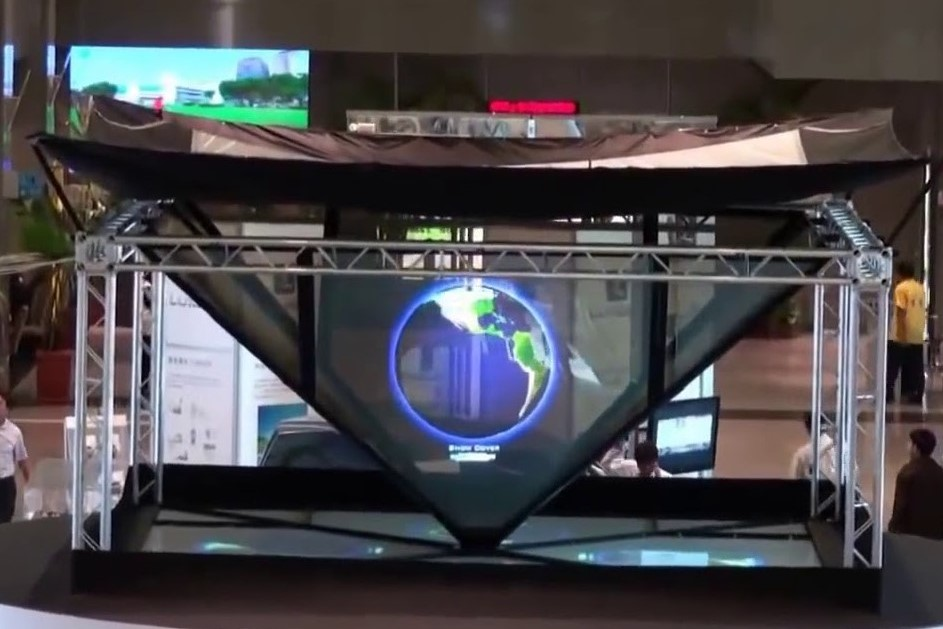
\includegraphics[width=0.47\textwidth]{img/bab2/p4_foto.jpg}}
		\hspace{0.1em}
		\subfloat[Video untuk piramida 4 sisi\cite{videop4}.]{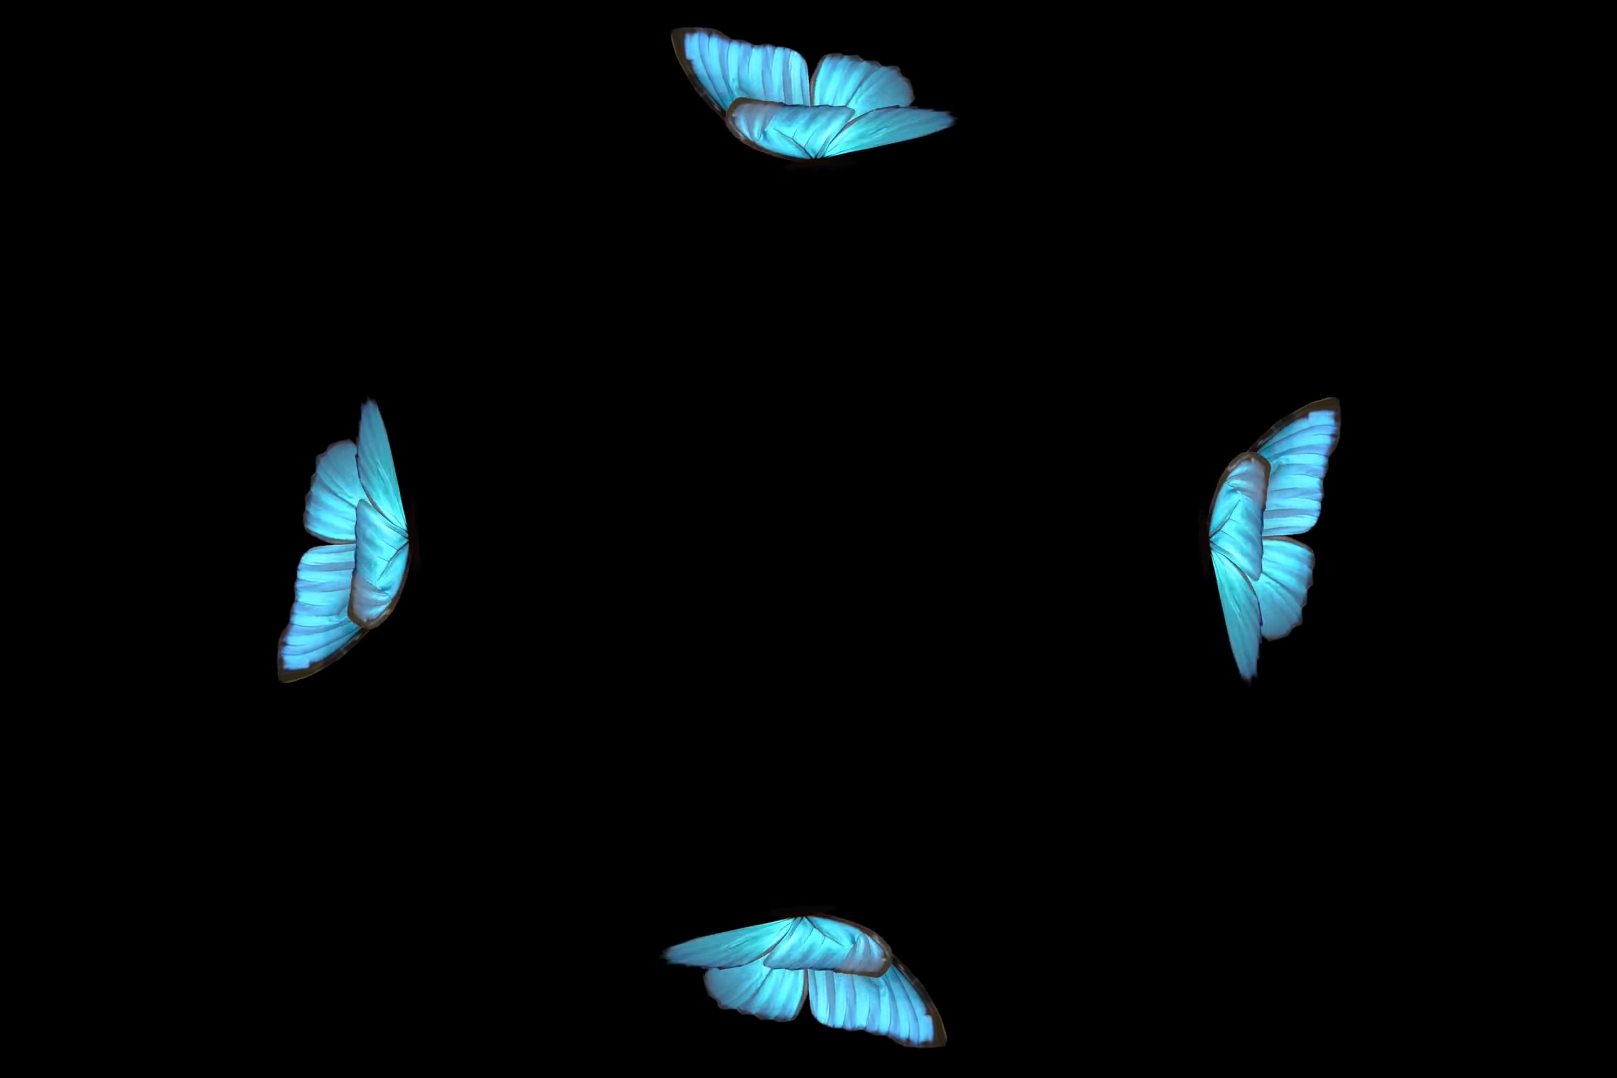
\includegraphics[width=0.47\textwidth]{img/bab2/p4_video.png}}
		\caption{Piramida 4 sisi}
		\label{fig:piramid4}
	\end{figure}
	
\vspace{2ex}

\section{\textit{Leap Motion Controller}}
\vspace{1ex}
	Leap Motion adalah sebuah perangkat yang dapat menggantikan \textit{mouse} maupun \textit{keyboard} tanpa harus menyentuhnya secara langsung. Leap Motion dihubungkan dengan komputer menggunakan USB 2.0  agar dapat membaca pergerakan tangan maupun jari yang diberikan oleh \textit{user}. Leap Motion berbeda dengan Kinect, dimana hanya informasi yang terbatas mengenai posisi tangan bukan \textit{depth map} seperti Kinect\cite{naidu2016hand}. Secara fisik, Leap Motion memiliki dimensi yang kecil yaitu 80 x 30 x 11,25 mm (3.1 x 1.2 x 0.5 inch) dengan bobot 3.2 gram. Dengan menggunakan 2 kamera monokrom yang berjarak 4cm dan 3 LED infrared, Leap Motion dapat melacak panjang gelombang 850 nanometer yang berada di luar spectrum cahaya tampak. Leap Motion memiliki jangkauan area sebesar 60 cm (2 ft) di atas \textit{controller}, 60 cm (2 ft) dengan sudut 150° untuk lebar setiap sisinya, dan 60 cm (2 ft) dengan sudut 120° untuk kedalaman setiap sisinya. Sedangkan \textit{interaction box} dalam sistem koordinatnya dapat menjangkau seluas 0.266 m³ (8 ft³) dengan bentuk piramida terbalik\cite{leapmotion_ds}. Keduanya dapat dilihat pada gambar \ref{fig:lm_int}.
	\begin{figure} [H]
		\subfloat[\textit{Interaction Area}\cite{leapmotionblog}.]{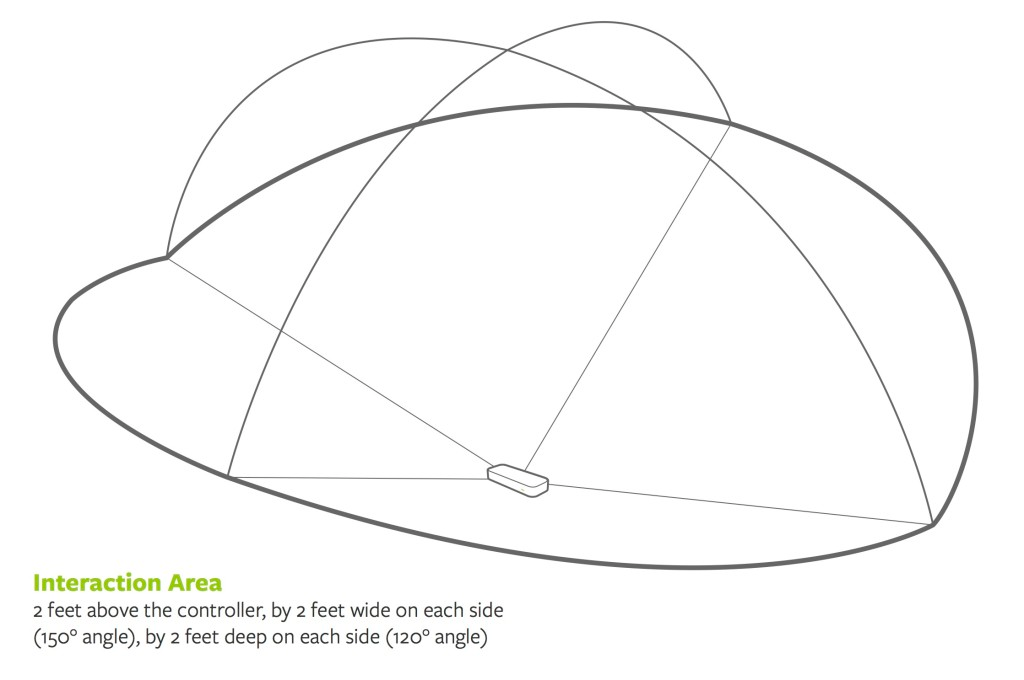
\includegraphics[width=0.47\textwidth]{img/bab2/lm_intarea.png}}
		\hspace{0.1em}
		\subfloat[\textit{Interaction Box}\cite{leapmotiondev}.]{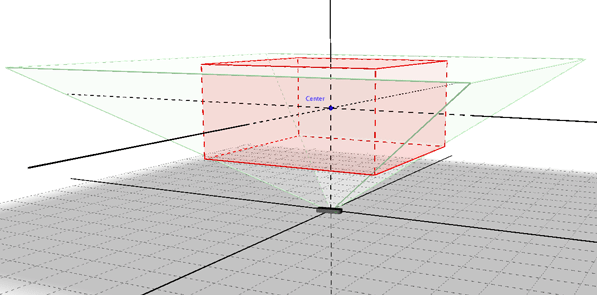
\includegraphics[width=0.47\textwidth]{img/bab2/lm_intbox.png}}
		\caption{Area yang dijangkau Leap Motion.}
		\label{fig:lm_int}
	\end{figure}
	Leap Motion dapat mengenali 27 bagian dari \textit{hand object elements} yang ditunjukkan pada gambar \ref{fig:handobject}. Elemen ini yang membuat Leap Motion dapat mengenali posisi tangan hingga dapat membaca \textit{motion} dan \textit{gesture}. \textit{Motion} atau pergerakan tangan didefinisikan sebagai \textit{continuous hand movements} yaitu memperkirakan posisi terhadap perubahan waktu, di antaranya \textit{scale}, \textit{rotation}, dan \textit{translation}. \textit{Gesture} didefinisikan sebagai perubahan pola yang dapat mentrigger aksi tertentu, di antaranya \textit{swipe}, \textit{circle}, dan \textit{tap}. Leap Motion bekerja dengan cara menangkap \textit{grayscale stereo image} yang dipisahkan berdasarkan kameran kanan dan kiri. Data tersebut disimpan dalam memori internalnya dan menjalankan penyesuaian resolusi. Kemudian dikirimkan via USB menuju Leap Motion Software untuk diolah datanya.
	\begin{figure} [H]
		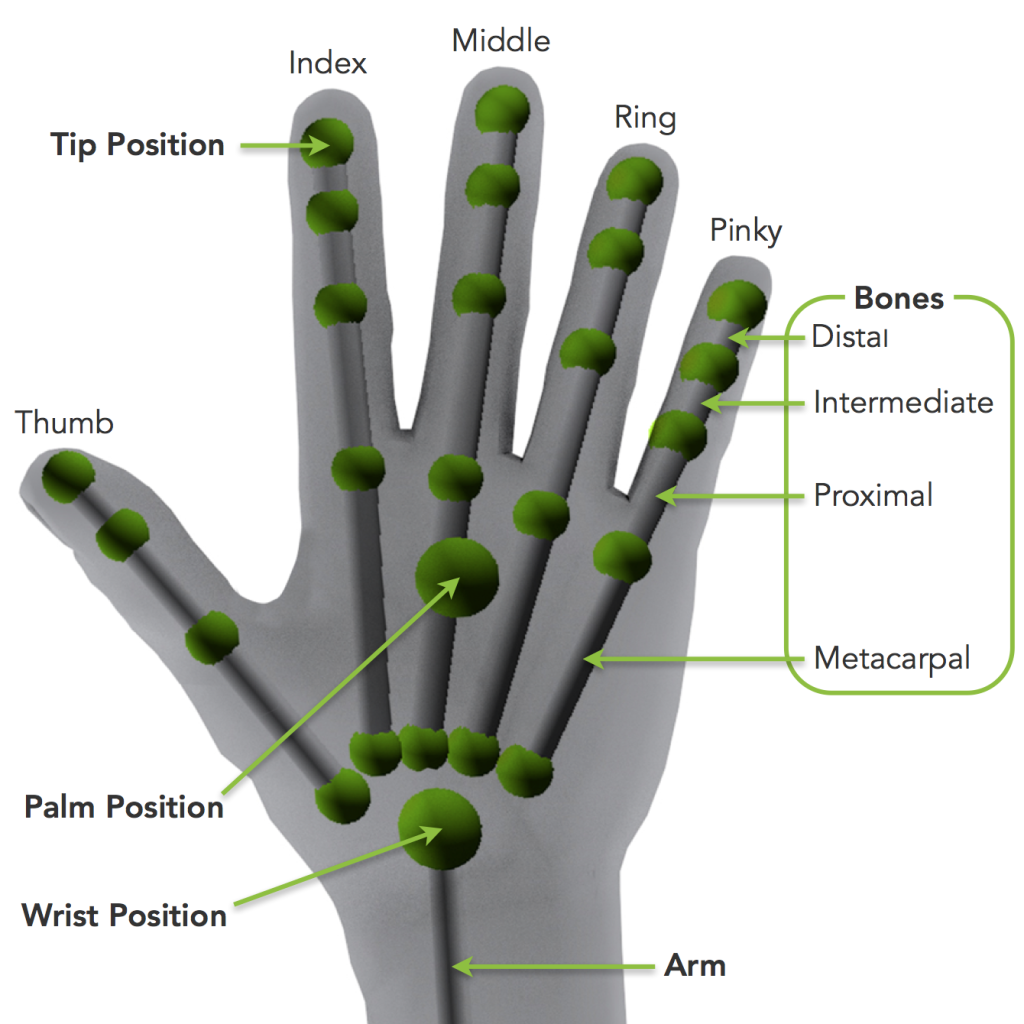
\includegraphics[scale=0.25]{img/bab2/handobject.png}
		\caption{\textit{Hand object elements} pada Leap Motion.}
		\label{fig:handobject}
	\end{figure}
\vspace{2ex}
